%******************************************************************************************************
\chapter[Introduction]{Quantifying Uncertainty of Computer Model: Forward and Backward}\label{ch:intro}
%******************************************************************************************************

% Introductory Paragraphs
\begin{quote}
	``All models are wrong but some are useful -- George Box''
\end{quote}
Perhaps. The quote by Box perhaps succinctly describes has been long used as.
Although indeed thermal-hydraulics co their use remains central in the .
There are reasons to be optimistic.

% Overview of the chapter
This opening chapter intends to introduce briefly the importance, the use and the challenges of using system code for simulating \gls[hyper=false]{th} behavior of \gls[hyper=false]{npp} in the context of its safety analysis.
Section~\ref{sec:intro_computer_simulation} starts with basic definitions of relevant terms used throughout the thesis before moving on to a brief introduction to safety analysis and thermal-hydraulics system code.
Uncertainty analysis of \gls[hyper=false]{th} system code is first discussed in Section~\ref{sec:intro_uncertainty_quantification}, outlining the background and the context of the doctoral research.

% Objectives, Scope, and Statistical Framework
Section~\ref{sec:intro_objectives_and_scope} then describes the statement of the problem, the objectives, and the scope of the research.
This thesis proposed a methodology comprises of sequential steps to analyze a computer model (i.e., \gls[hyper=false]{th} system code) with the overall goal of quantifying the uncertainty associated with the model parameters based on experimental data.
It consolidates and adapts recent developments of in the applied statistics literature.
In relation to that, Section~\ref{sec:intro_statistical_framework} provides a broad, and by no means exhaustive, overview of the research landscape on each of the proposed steps.
Finally, Section~\ref{sec:intro_thesis_structure} concludes the chapter by outlining the structure of the thesis.

\section{Computer Simulation and Safety Analysis of Nuclear Power Plant}\label{sec:intro_computer_simulation}
Illo principalmente su nos. Non message \emph{occidental} angloromanic
da. Debitas effortio simplificate sia se, auxiliar summarios da que,
se avantiate publicationes via. Pan in terra summarios, capital
interlingua se que. Al via multo esser specimen, campo responder que
da. Le usate medical addresses pro, europa origine sanctificate nos
se.
%*************************************************************************************************************************
\section{Uncertainty Quantification in Nuclear Engineering Thermal-Hydraulics}\label{sec:intro_uncertainty_quantification}
%*************************************************************************************************************************

% Introductory Paragraph
Before continuing the discussion of uncertainty analysis of code predictions, it will be worthwhile to define some additional terminologies to avoid later confusion.

In making a connection with the notion of \emph{simulator} introduced in Section~\ref{sec:intro_computer_simulation}, 
recall that from Fig.~\ref{fig:ch1_th_system_code} an \emph{input deck} is distinct from the code itself.
Fig.~\ref{fig:ch1_simulator_io} depicts the notion of simulator of a thermal-hydraulics system in a more generic way, as an input/output model.
\begin{figure}[bth]	
	\centering
	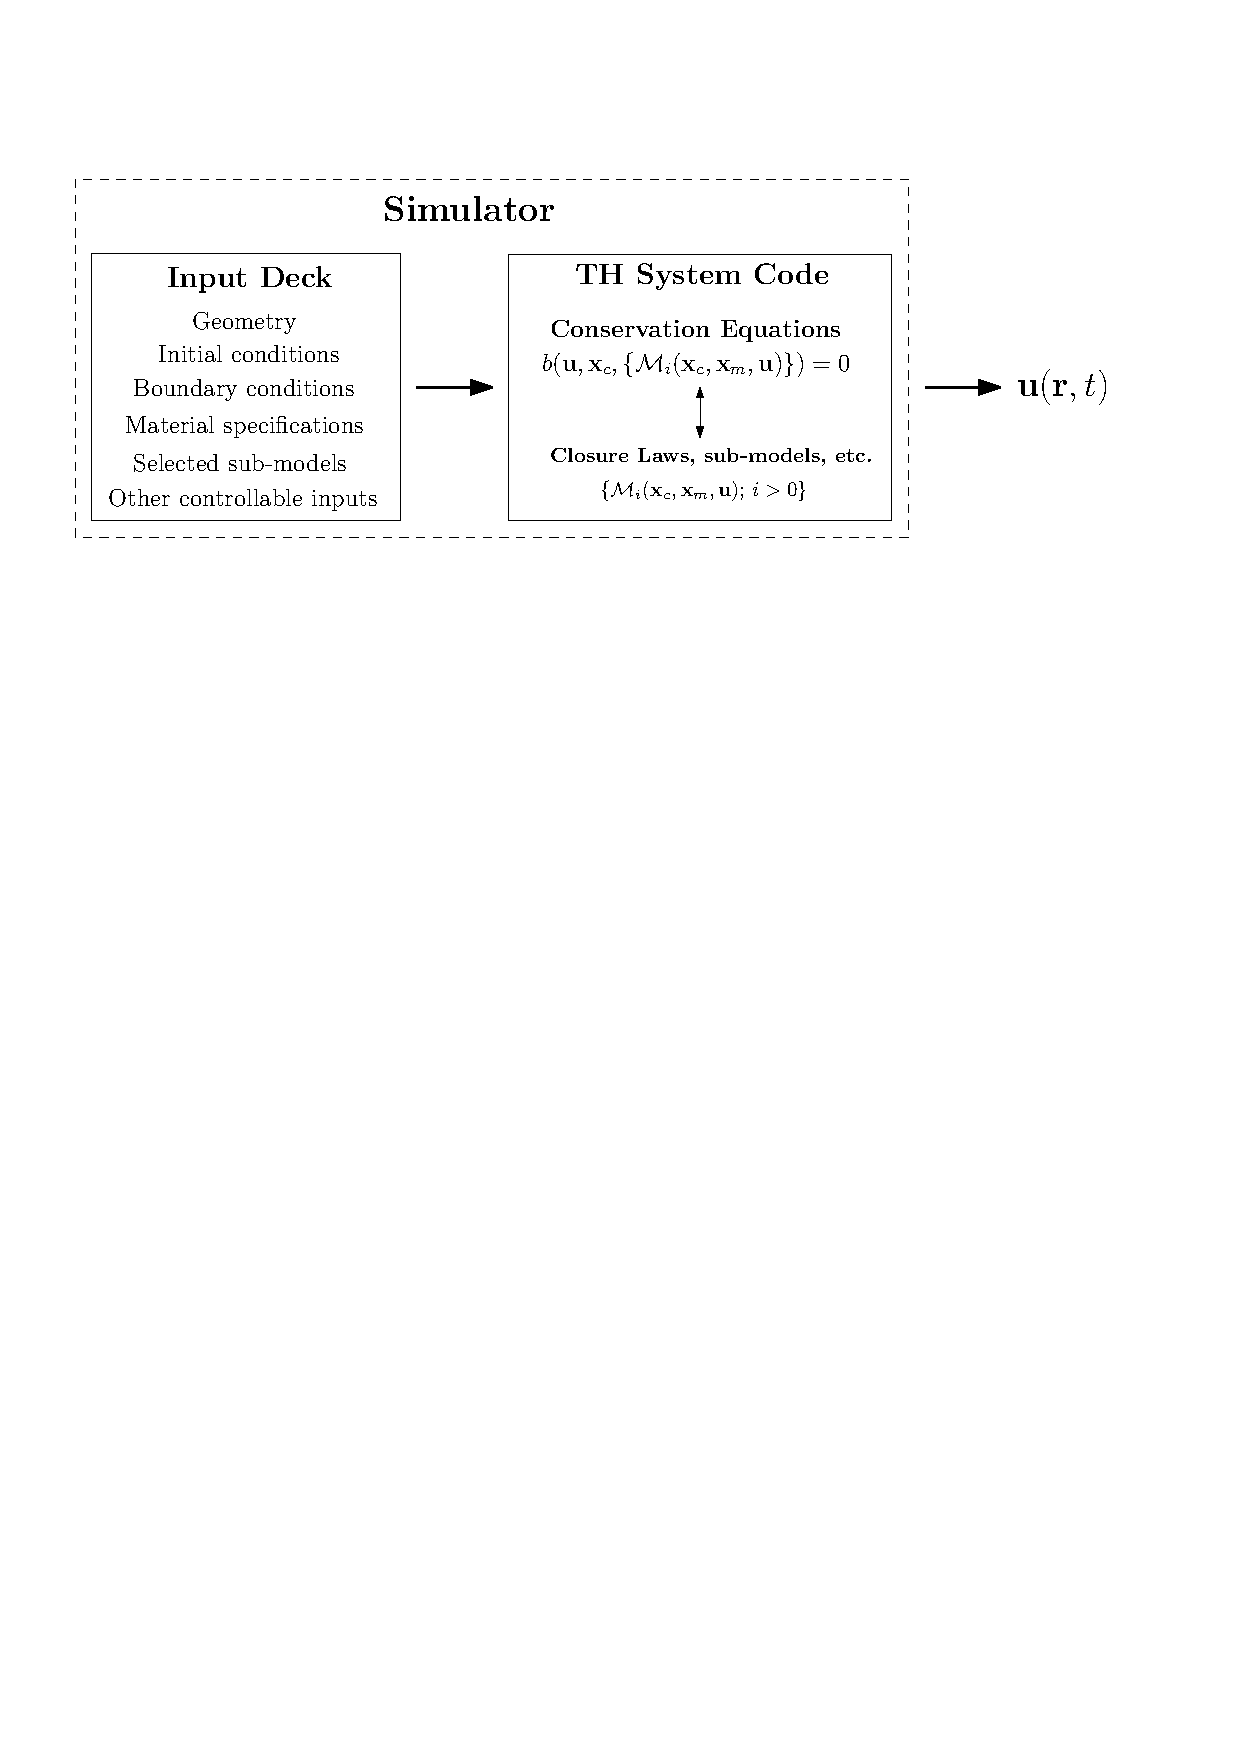
\includegraphics[width=\textwidth]{../figures/chapter1/figures/simulator_io}
	\caption[Simplified illustration of a simulator as an input/output model.]{Simplified illustration of a simulator as an input/output model.}
	\label{fig:ch1_simulator_io}
\end{figure}

Indeed, an input deck defines a specific problem (i.e., system) of interest.
It includes the specifications for geometrical configuration (i.e., the nodalization), choice of material and fluid involved, as well as initial and boundary conditions.
It may also include the setting for the numerical solver.
\marginpar{Controllable inputs and model parameters}
Some of those specifications (such as the boundary conditions, etc.) are parametrized and constitutes \emph{controllable inputs} denoted by $\bm{x}_c$ that define a particular instance in which the simulator is to be used\footnote{later on, \emph{controllable} inputs correspond to the parameters whose counterparts in a physical experiment which can be controlled by the experimentalist.}.
The conservation equations of the code are closed with additional set of closure laws (and other sub-models) $\mathcal{M}_i(\bm{x}_c, \bm{x}_m, \bm{u})$.
These closure laws are, in turn, parametrized by a set of model specific parameters denoted by $\bm{x}_m$ which is referred to as the \emph{physical model parameters}.
Note that both the controllable inputs and the physical model parameters are considered by the code simply as \emph{inputs}.
 
Specifying the input deck, as far as user is concerned, completely defines the problem and the code will solve the conservation equations $b$ which output the dynamic state of relevant physical variables $\mathbf{u}(\bm{r}, t)$ (e.g., fluid pressure, temperature, wall temperature, etc.). 
In practice, these ``raw'' outputs are further post-processed to obtain the so-called \glspl[hyper=false]{qoi} the are relevant to the problem at hand (e.g., max. temperature, max. pressure, onset time, etc.).

%--------------------------------------------------------------------------
\subsection{Forward Uncertainty Quantification}\label{sub:intro_uq_forward}
%--------------------------------------------------------------------------

% Best-estimate, limitation
As explained, best-estimate analysis uses more realistic modeling assumptions for analyzing transient behavior of \gls[hyper=false]{npp}.
It attempts as realistically as possible to describe the behaviors of the relevant physical processes that occur during the plant transient.
And yet, even the best available understanding of the physical process is still limited.
Understanding of complex phenomena might not yet be adequate and data support for some processes can be very limited.
Simplifying assumptions, approximations, and expert judgments to some degree are unavoidable and still required to have a complete analysis.

% Best-estimate, plus uncertainty
Hence, best-estimate analysis has to be complemented with uncertainty analysis.
\marginpar{Best-estimate plus uncertainty}
The ultimate goal of uncertainty analysis is to associate code prediction with its uncertainty.
These combined quantities are then compared with certain safety limits (e.g., \gls[hyper=false]{pct}) to check whether the limits still fall outside the uncertainty band of the code prediction.

% Source of possible uncertainties
There are several known sources of uncertainty that render the prediction on $\bm{u}(\mathbf{r},t)$ and its derived quantities uncertain.
\marginpar{Sources of uncertainty}
The following are the sources of primary interest in the present research:
\begin{enumerate}

	\item \emph{Uncertainty associated with the controllable inputs}.
	In the case of a controlled experiment, these controllable inputs are supposed to be observed (and \emph{controlled}).
	However, such an observation might contain errors due to instrument imprecision and/or inherent variability. 
	When simulating a real accident scenario in a plant,
  some conditions of the plant parameters prior to the accident scenario (its initial conditions) can also be measured.
  In such a scenario, controllable inputs may also include parameters that are part of the assumptions underpinning the deterministic safety analysis (i.e., conservative vs. best-estimate).
  That is, it includes the degree of pessimism in the (assumed) boundary conditions, ranging from the availability of safety features to the constraints on their performance \cite{IAEA2002}.

  \item \emph{Uncertainty associated with the physical model parameters}.
	The value of the physical model parameters are often not known a priori.
	As such the uncertainty associated with them are epistemic in nature.
	They can either be estimated by using an experimental data from a calibration experiment or by expert judgment.
	
  \item \emph{Uncertainty associated with the physical models}.
	The physical models themselves are still approximations, even with perfectly known model parameters.
	If derived in a fully mechanistic manner, some important processes might be unaccounted for due to the inherent complexity and lack of knowledge (i.e., the case of \emph{missing physics}).
	On the contrary, if derived fully empirically, models might be derived separately from different elementary processes, while in the applications of the code multiple of such models are used in concert.
	Despite each being validated, it is fair to question the validity of models used in an ensemble.
	Any of the two points tends to cause a systematic bias on the code prediction, the extend of which is unknown and uncertain.
	As a result, this source of uncertainty is referred to as model \emph{bias}, \emph{inadequacy}, or \emph{discrepancy}.

\end{enumerate}

% Forward uncertainty quantification, Inputs as random variables
In statistical uncertainty analysis, the controllable inputs and physical model parameters are modeled as random variables ($\bm{\mathcal{X}}_c$ and $\bm{\mathcal{X}}_m$, respectively) equipped with \glspl[hyper=false]{pdf}.
\marginpar{Forward uncertainty quantification}
By transforming the random variable inputs, the simulator output becomes random variable as well
\begin{equation*}
	\bm{\mathcal{U}}(\bm{r}, t) = f(\bm{\mathcal{X}}_c, \bm{\mathcal{X}}_m;\bm{r}, t)
\end{equation*}
where $f$ represents the simulator as a mathematical function.
The \gls[hyper=false]{qoi} related to the random code outputs can be summarized by different integral quantities.
For instance, the mean of a \gls[hyper=false]{qoi} given by function $g$ is
\begin{equation*}
	\mathbb{E}[g] = \int\limits_{\mathbf{X}_c,\mathbf{X}_m} g(f(\bm{x}_c, \bm{x}_m;\bm{r}, t)) \, p(\bm{x}_c, \bm{x}_m) \, d\bm{x}_c \, d\bm{x}_m
\end{equation*}
where $p(\bm{x}_c, \bm{x}_m)$ denotes the joint \gls[hyper=false]{pdf} for the input parameters.

Using \gls[hyper=false]{mc} technique, samples are generated from their respective distributions and are used to run the code multiple times.
Afterward, the resulting code outputs (raw or post-processed), are summarized to obtain the uncertainty measure of the prediction.
In other words, the uncertainties in the controllable inputs and physical model parameters are \emph{propagated forward} through the code to quantify the uncertainty of the predictions as shown in Fig.~\ref{fig:ch1_simulator_uq_forward}.
The practice of propagating parametric uncertainty by \gls[hyper=false]{mc} is widely accepted in the nuclear engineering thermal-hydraulics community \cite{Lellouche1990,Glaeser1994,Glaeser2008}.
\begin{figure}[!bth]	
	\centering
	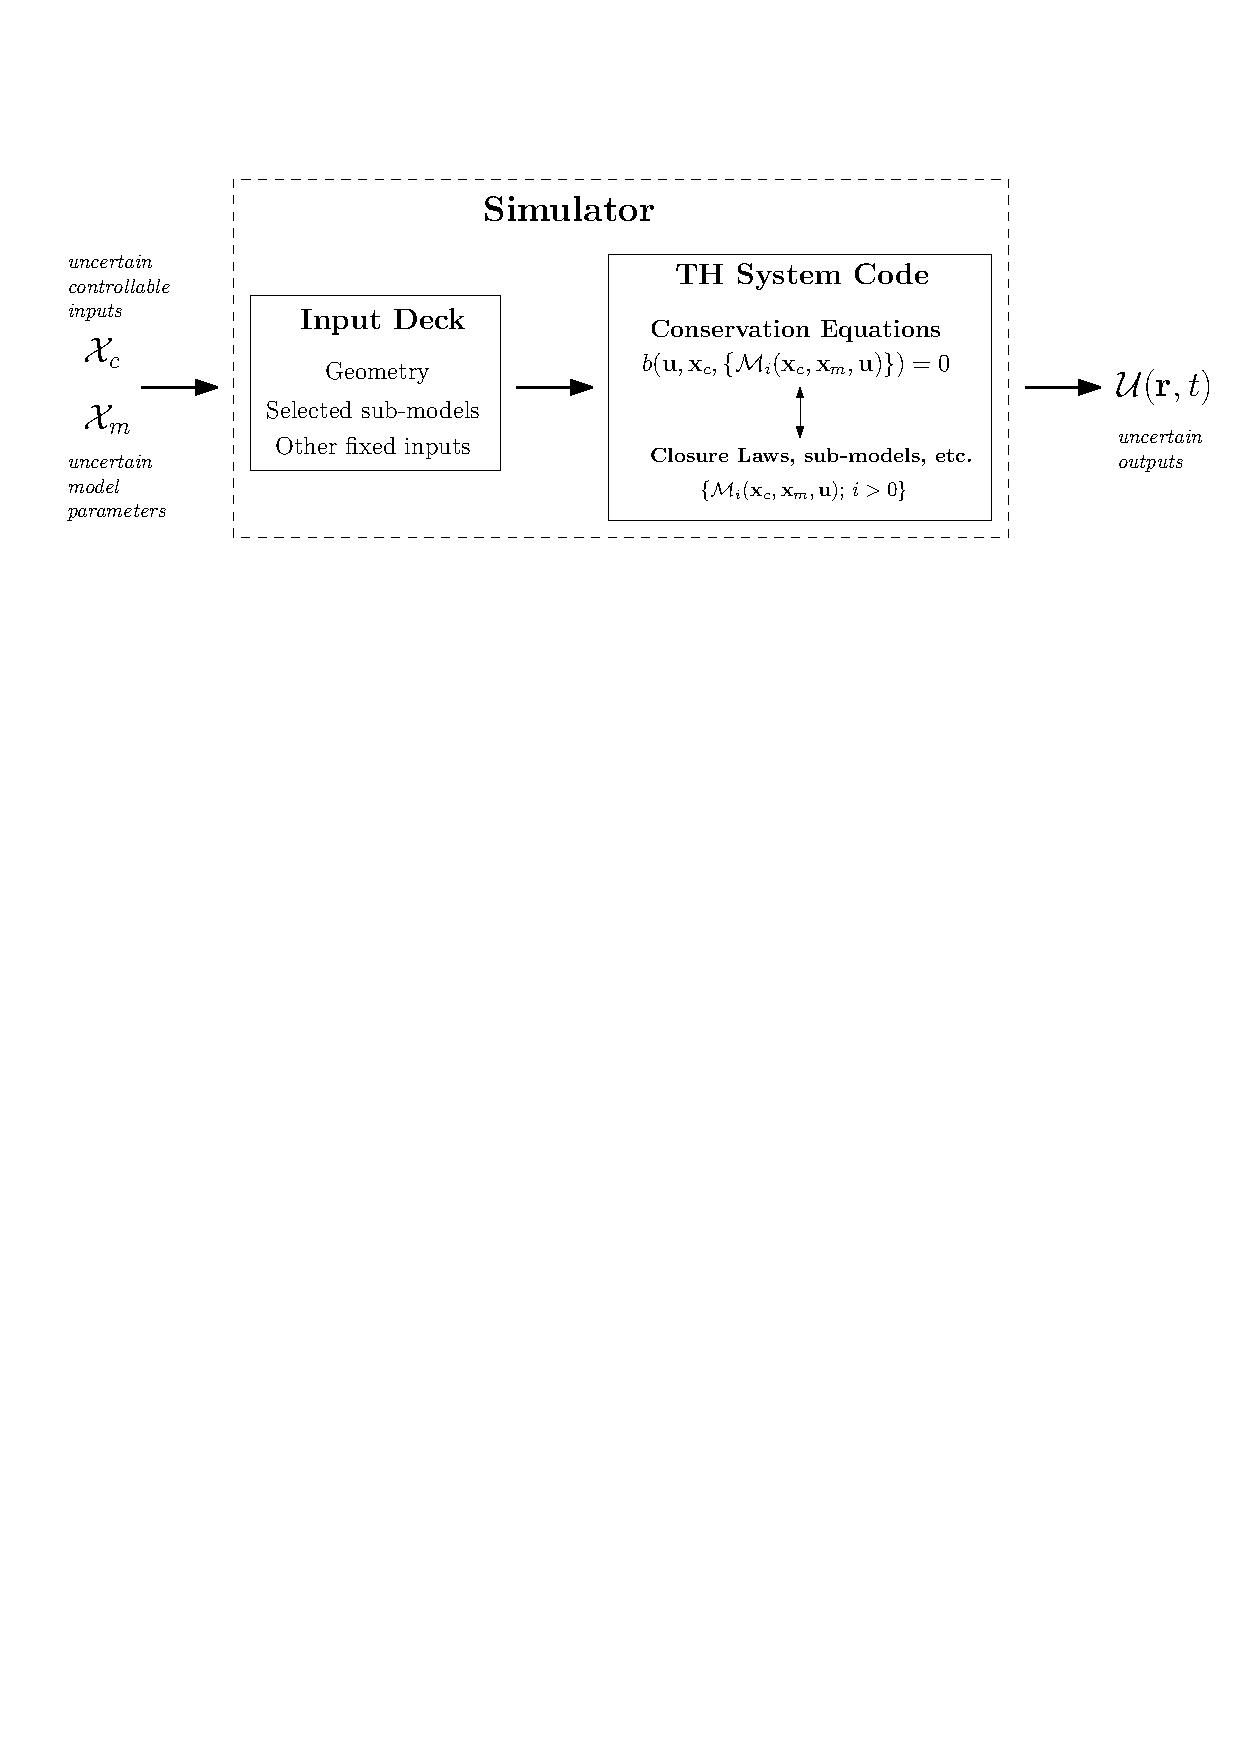
\includegraphics[width=\textwidth]{../figures/chapter1/figures/simulator_uq_forward}
	\caption[Simplified flowchart of forward uncertainty quantification of a simulator prediction.]{Simplified flowchart of forward uncertainty quantification of a simulator prediction. Notice that the simulator has been parametrized by the controllable inputs and physical model parameters, each of which are represented as a random variable.}
	\label{fig:ch1_simulator_uq_forward}
\end{figure}

% Source of uncertainty, initial and boundary condition
The forward uncertainty quantification explained above deals with the parametric uncertainty associated with the important parameters of the simulator, both for the controllable inputs and the physical model parameters.
As a result, representing the inputs of the simulator as random variables is the key in the forward uncertainty quantification of system code.

%-------------------------------------------------------------------------------------
\subsection{Inverse (Backward) Uncertainty Quantification}\label{sub:intro_uq_inverse}
%-------------------------------------------------------------------------------------

% Model parameters
A lot has been said about the origin of the uncertainty associated with the controllable inputs.
The physical model parameters, however, are conceptually different.
\marginpar{Model parameters}
The physical models referred to in this thesis are usually represented either in the form of correlation, phenomenological model, or a mixed between the two extremes (see Section~\ref{sub:intro_th_system_code}).
The parameters associated with the models can either represent physically meaningful quantities or not (This distinction will be revisited in Chapter~\ref{ch:bayesian_calibration}).
The uncertainty on these parameters depends on the parameters origin.
For instance, in an empirical model the model parameters are the curve-fitting parameters and its uncertainty can be associated with the dispersion of the data.

% Representativity for NPP application
However, it is worth considering that many such models, be it empirical or mechanistic, were originally derived based on simple systems that did not, strictly speaking, reflect the flow conditions in an \gls[hyper=false]{lwr} (e.g., heated tube vs. rod bundle, low pressure vs. high pressure, etc.) \cite{Bestion2008}.
\marginpar{Separate Effect Test Facilities}
Thus, to reflect more on the conditions of flow in the reactor transient to be simulated,
experiments with well-specified conditions are conducted at \glspl[hyper=false]{setf}, facilities aimed at reproducing a particular safety-relevant phenomena during transient at a particular part of the reactor \cite{DAuria2012}.

The data sets from \glspl[hyper=false]{setf} are then used to assess the corresponding model (and possibly multiple models).
In the assessment,
some parameters in the models are adjusted to match the experimental data \cite{Barre1990}.
\marginpar{Calibration against Separate Effect Test Facilities}
Alternatively, additional free parameters can also be introduced in the models to serve the same purpose \cite{Bestion2008}.
That is, the parameters are tuning parameters and become measures of the models inadequacy in reproducing the data.
Ultimately, some kind of optimal values for the parameters are estimated and implemented in the code.

% Origin of uncertainty
In light of this, it can be argued that the uncertainty associated with such parameters stems from the fact that the calibration was conducted only on limit set of data obtained from a selected \gls[hyper=false]{setf}.
Different \glspl[hyper=false]{setf} for the same phenomena exist, covering wide ranges of flow configurations and experimental boundary conditions.
It is fair to ask if the calibrated value will hold if the calibration were to be conducted in other \glspl[hyper=false]{setf} for the same phenomena.
Additionally, as tuning parameters, expert-judgment is also often used to estimate the uncertainty, measuring the degree of expected model performance through how much the model parameter is allowed to vary.

% Inverse uncertainty
To derive the uncertainty associated with the model parameters obtained described above,
the problem can be posed as an inverse problem.
\marginpar{An inverse problem}
In this setting, given a set of experimental data $\{\mathbf{D}\}$ taken with known controllable inputs $\mathbf{x}_c$, the task is then to infer the value of the \emph{unobserved} parameters in the physical model used to predict the same quantity as the experimental data.
To avoid excessive bias to the calibration data, it is important here to acknowledge the observation errors of the observed experimental data and the controllable inputs, and the possible systematic bias of the associated models.

% Bayesian framework
In a probabilistic setting, a way to make an inference of unobserved parameters based on observed data is
\marginpar{Inverse uncertainty quantification}
through the Bayes' theorem,
\begin{equation*}
	p(\bm{x}_m\,|\,\{\mathbf{D}\},\mathbf{x}_c) = \frac{p(\{\mathbf{D}\}\,|\,\bm{x}_m, \mathbf{x}_c) \cdot p(\bm{x}_m)}{\int p(\{\mathbf{D}\}\,|\,\bm{x}_m, \mathbf{x}_c) \cdot p(\bm{x}_m)\,d\bm{x}_m}
\end{equation*}
where the left-hand side of the equation is the posterior probability density conditioned on the observed data $\{\mathbf{D}\}$ and controllable inputs $\mathbf{x}_c$.
The right-hand side constitutes of the likelihood function $p(\{\mathbf{D}\}\,|\,\bm{x}_m, \mathbf{x}_c)$ (probability of observing data given the parameters), the prior of the model parameters $p(\bm{x}_m)$ (the initial state of knowledge regarding the parameters values before observing the data),
while the denominator is a normalizing constant such that the posterior is a valid \gls[hyper=false]{pdf} (that is, it integrates to one)\footnote{Note that the formulation assumes the controllable inputs $\mathbf{x}_c$ are fully known. If they are considered uncertain, such as in the case of variability, then a prior probability can be put on them as well.}.
The posterior represents the knowledge one has on the model parameters values conditioned on the data under the modeling assumption.
Fig.~\ref{fig:ch1_simulator_uq_inverse} depicts a simplified flowchart of the inverse quantification.
\bigfigure[pos=tbhp,
           opt={width=1.0\textwidth},
           label={fig:ch1_simulator_uq_inverse},
           shortcaption={Simplified flowchart of inverse uncertainty quantification of model parameters.}]
{../figures/chapter1/figures/simulator_uq_inverse}
{Simplified flowchart of inverse quantification for model parameters of a simulator.}

The formulation and computation of the posterior above can be seen as a calibration exercise.
That is, it seeks to adjust the model parameters such that it is consistent with the observed data (i.e., calibration data) under the assumed likelihood and the prior.
\marginpar{Statistical calibration}
However, instead of obtaining a single estimated value (or values in case of multiple parameters), the resulting posterior is a \gls[hyper=false]{pdf}, conditioned on the observed data.
In relation to the aforementioned expert-judgment for the estimating the parameters uncertainty, the approach uses the experimental data to better inform the prior expectation about the model parameters values.
The posterior \gls[hyper=false]{pdf}, in turn, can be used in uncertainty propagation to quantify the uncertainty on the prediction made outside the calibration data set.

% Connection to PREMIUM Benchmark
The importance of characterizing the uncertainty in the physical models parameters was acknowledged by the \gls[hyper=false]{wgama} of the \gls[hyper=false]{oecd}/\gls[hyper=false]{nea}.
This led to the \gls[hyper=false]{premium} project.
Its main goal is to report the state-of-the-art methodologies to quantify the uncertainty in the physical models parameters.
The following will briefly describe the project and highlight the selected main lessons learned from the author's perspective through his participation on behalf of the \glsfirst[hyper=false]{psi} \cite{Wicaksono2016a}.

%-------------------------------------------------------------
\subsection{OECD/NEA PREMIUM project}\label{sub:intro_premium}
%-------------------------------------------------------------

% Introductory paragraph
The \gls[hyper=false]{premium} project was an activity launched by the \gls[hyper=false]{oecd}/\gls[hyper=false]{nea} with the aim to advance the methods for quantifying the uncertainties associated with the physical model parameters in \gls[hyper=false]{th} system codes.
It was the continuation of the previous project \gls[hyper=false]{bemuse}, which concentrated on the propagation and sensitivity analysis of the input uncertainties in large scale simulation (\gls[hyper=false]{lbloca}).
The main finding of \gls[hyper=false]{bemuse} can be found in \cite{Perez2011}.
The emphasis of the \gls[hyper=false]{premium} benchmark was placed on the derivation of the model parameters uncertainty and their validation.

% Scope of the Project
The scope of the project was limited to the simulation of the phenomenon of core reflood and quenching under conditions representative of a \gls[hyper=false]{pwr} large break \gls[hyper=false]{loca}.
Experimental data from two \glspl[hyper=false]{setf} was made available for the purpose of uncertainty quantification of the model parameters as well as validation.
For the model parameters uncertainty quantification, the data from the \gls[hyper=false]{feba} reflood facility was used.
Although, the experimental data were taken at several controllable inputs (i.e., boundary conditions) in practice calibration was conducted using only one.
The derive uncertainties were then propagated and compared with the experimental data from other experimental runs of \gls[hyper=false]{feba} and from another reflood facility (PERICLES).
Thus the main goal of the project followed the approach of statistical uncertainty analyses explained above.

% Phase
Sixteen organizations from $11$ different countries participated in the $4$-year project ($2012$--$2016$) using $6$ different \gls[hyper=false]{th} system codes.
Each participant employing a chosen simulation code and methodology had to contribute to the $5$ following phases of the benchmark:
\begin{enumerate}
	\item \textsc{Phase 1}: Description of the selected simulation code and methodology.
  \item \textsc{Phase 2}: Identification of the uncertain parameters that are most relevant to \gls[hyper=false]{pwr} \gls[hyper=false]{loca} reflooding simulations.
  \item \textsc{Phase 3}: Quantification of the uncertainties in the parameters, using available data from the \gls[hyper=false]{feba} experiment.
  \item \textsc{Phase 4}: Propagation of the quantified uncertainties as part of a blind benchmark exercise based on data from the PERICLES experiment.
  \item \textsc{Phase 5}: Contribution to the analysis and synthesis of the benchmark results.
\end{enumerate}
During the course of the project up to its conclusion, three \gls[hyper=false]{oecd}/\gls[hyper=false]{nea} reports have been published \cite{Kovtonyuk2015, Reventos2016,Sanz2017}.
Details can be found in the reports.
The following will describe briefly some of the lessons learned from \gls[hyper=false]{premium} that of relevance to the present study.

% Lessons learned
\gls[hyper=false]{premium} provided state-of-the-art (as of $2015$) uncertainty quantification methods for \gls[hyper=false]{th} system codes.
It emphasized methodological issues that are yet to be overcome.
Some of these issues, such as the identification of important parameters, extrapolation of quantified results, scaling, and nodalization were already raised in the $1994$ review studies on uncertainty methods for \gls[hyper=false]{th} codes sponsored by the European Commission \cite{Forge1994}.
At the conclusion of \gls[hyper=false]{premium}, these issues are still considered open problems.

% The problem of systematic identification of important parameters
First, there was an apparent lack of consensus among participants (and thus, the community) for a systematic identification of important parameters in \gls[hyper=false]{th} simulation models.
\marginpar{Identification of important parameters}
Guidelines were indeed provided, but each participants eventually came up with their own selection criteria and methodology, some still relied solely on graph comparison of outputs from changing one parameter at a time \cite{Kovtonyuk2015}.

Although complete exclusion of expert judgment is not feasible (nor advised), it is useful to take benefit from the progress made in the computer experiment community.
For instance, the Morris screening method can be useful in the initial parameter identification and importance ranking process by making the analysis more systematic and robust.
The method can provide smooth transition from the more familiar one-at-a-time method adopted by most participants.
Furthermore, there was a valid issue raised by a participant regarding the possibility of ``complicated'' code response from simultaneous parameters perturbation \cite{Wicaksono2015}.
This can be interpreted perhaps as parameter interaction in the literature.
In this case, \gls[hyper=false]{gsa} methods can help in the investigation about its presence. 

% The problem of calibration and overfitting
Secondly, there was a slight disagreement between participants regarding the use of \emph{calibrated parameter}.
This notion stemmed from the use of a Bayesian method (the so-called CIRC\'E \cite{Crecy2001,Reventos2016}, a method based on maximum likelihood approach under linear assumption coupled with normal prior for the parameter) to update the prior distribution of the model parameter such that the resulting posterior distribution yields the closest agreement with the experimental data.
\marginpar{Calibrated parameter and best-estimate code}
Furthermore, the nominal value of the model parameter was allowed to shift following the updated central measure of the posterior.
Such practice of calibration was questioned because the best-estimate code used was, in fact, already calibrated on the basis of larger experimental database over decades of verification and validation (V\&V) activities.
In other words, the calibration over a very limited set of the \gls[hyper=false]{feba} tests would undermine the built-in (calibrated) models already in place.

That was a valid point of contention.
The results of applying CIRC\'E were mixed. 
On one hand the experimental data from the \gls[hyper=false]{feba} experiment allowed CIRC\'E to reduce the initial uncertainty on the parameters and simultaneously improved the nominal case prediction.
On the other hand, when the updated parameters were used in the uncertainty propagation of a \gls[hyper=false]{feba} test, the narrow uncertainty band on the prediction failed to cover some part of the experimental data.
Moreover, when the same updated parameters were used in the blind uncertainty propagation for another facility there results were poor: poor nominal case prediction (note that the nominal parameters values were allowed to be updated) and too narrow uncertainty without covering the experimental data \cite{Wicaksono2016a,Sanz2017}.

This indicated a symptom of \emph{overfitting} where the uncertain parameters were calibrated strongly on one data set and thus became very sensitive to a change of data set.
\marginpar{Overfitting and extrapolation}
The narrow uncertainty obtained indicates that the calibration procedure converged to a ``wrong'' values and thus was not applicable to extrapolation.

While the Bayesian approach makes sense for parameter calibration, updating its value in light of new data,
its application might require more examination on the additional sources of uncertainty.
It also makes sense to acknowledge the extensive V\&V activities that serve as the basis of \gls[hyper=false]{th} system codes;
observing one additional data set should not render previous results invalid right away.
Thus it remains an open question how to compromise between learning from the new data and preserving what has been learned before.

% The use of metamodel
Finally, there is a natural reluctance among the participants to embrace more advanced methods requiring less assumptions (e.g., normal prior of the parameters, linearity between outputs and parameters, etc.) but with more computational cost (i.e., more code runs) that are available in the recent literature.
\marginpar{The use of metamodel}
The use of metamodel can help in alleviating such computational restriction\footnote{It is not, however, cost-free as will be explained in more detail in Chapter~\ref{ch:gp_metamodel}.}, insofar that the error incurred by the use of metamodel can be accepted.
Strictly speaking, the community is not unfamiliar with the use of metamodel (a fast approximating function as a substitute of running the code) for uncertainty analysis, especially in the context of uncertainty propagation\footnote{It was initially used for the estimation of \gls[hyper=false]{pct} probability distribution from uncertainty propagation in the context of safety margin evaluation of \gls[hyper=false]{lbloca} scenario \cite{Boyack1990}.}.
However, in the context of inverse uncertainty quantification, none of the participant took the benefit of using metamodel and relaxed some of the assumptions in calibration.

\newpage
%*********************************************************************************
\section{Objectives and Scope of the Thesis}\label{sec:intro_objectives_and_scope}
%********************************************************************************* 

With a larger context provided above,
this section presents briefly and specifically the statement of the problem,
followed by the objectives as well as the scope of the present doctoral research.

%--------------------------------------------------------------------------
\subsection{Statement of the Problem}\label{sub:intro_statement_of_problem}
%--------------------------------------------------------------------------

% Introductory Paragraph
The development of closure laws for reflooding described in \cite{Nelson1992,USNRC2012} showed the difficulties and the amount of assumptions used.
In a nutshell, system code development is an effort to consolidate correlations and mechanistic models, to create a phenomenological-based simulation code that can provide best-estimate results.
This consolidated effort results in a code that can simulate wide range of transients foreseen in nuclear power plant operation in a best-estimate manner.
Alas, to come up with a consistent set of closure laws is a great challenge for code developers.

% Closure Laws Difficulty, Conceptual
The closure laws required to close the two-fluid model pose particularly difficult challenges \cite{Wulff2007}.
For instance, to have a correlation of heat transfer between the wall and the fluid, temperature data from each of the constituents are needed (i.e., the wall, the liquid phase, and the gas phase).
But measuring temperature of the individual phases in an arbitrary interfacial topology has its own technical difficulties to the extend that no such data exists or available to be implemented in the closure laws.
Additionally, the experiments to obtain hydrodynamic closure laws (e.g., interfacial friction factor, wall friction factor, etc.) were generally carried out in adiabatic conditions.
As a result, this excludes the coupling of any heat transfer phenomena between the phases and the wall in such correlation.

% Closure Laws Difficult, Practical
Furthermore, during the development of a simulation code, programming considerations also came into the picture.
For robustness, simplification is often required and continuity is enforced.
Transitionary flow regime between two known (observed) flow regimes for which experimental data is not available is modeled to be the average of the two bounding regimes.
Different code development, which used different assumptions and experimental database, comes up with different set of closure laws with their own parametrization (see for instance \cite{Nelson1992} for TRAC code and \cite{Bestion1990} for CATHARE code).
Several authors have expressed their concerns about the uncertainty stemming from the closure laws \cite{Wulff2007,Petruzzi2008a,DAuria2012}.

% an Illustration
As an example of the point given above, consider that in the \gls[hyper=false]{trace} code, after some derivations the interfacial drag coefficient closure law in the inverted slug flow regime $C_{i,\text{IS}}$ is given by,
\begin{equation*}
	C_{i,\text{IS}} = \hat{x}_{m,\text{SET}} \times \frac{1}{24} \frac{\rho_g}{\text{La}} \frac{(1-\alpha)}{\alpha^{1.8}} \,\,\,;\,\,\, \hat{x}_{m,\text{SET}} = 0.75 
\label{eq:intf_drag_isf}
\end{equation*}
where $\rho_g$ is the density of the gas phase;
$\text{La}$ is the Laplace number;
$\alpha$ is the void fraction;
and $\hat{x}_{m,\text{SET}}$ is a fitting parameter.

There are several remarks that can be made about the closure law given above.
First, the second term in the right-hand side was derived from experimental data but not directly.
In the inverted slug regime, saturated liquid core breaks up into ligaments.
These ligaments are \emph{assumed} to take form as prolate ellipsoid.
The drag coefficient of distorted droplet experimental database is then \emph{assumed}.
Then to take into account the multi-particle effect, the coefficient is divided by the void fraction $\alpha$ raised to the power of $1.8$ (this, in turn, was taken from experimental data of inertial regime).
Lastly, the first term of the equation, $\hat{x}_{m,\text{SET}} = 0.75$ was put \emph{to match}, \emph{to calibrate against} the experimental data from the FLECHT-SEASET reflood experimental facility.
This first term, although clearly \emph{non-physical} in nature, is an important tuning parameter of the model nevertheless.
Its uncertainty should be considered in uncertainty analysis, especially when reflood is expected to occur.
Yet, no statement regarding the associated uncertainty is given.
Several other such terms exist \cite{USNRC2012}. 

% Statement of Problem
As illustrated above, it is clear that models in thermal-hydraulics system code, to a certain extent, flawed.
Various experimental programs were carried out to gain better understanding of important phenomena,
and to validate (and, as noted, to calibrate) the models.
Series of the experiments, carried out in \glspl[hyper=false]{setf} with a well-specified boundary conditions were aimed to reproduce limited part of the transient in a selected component following a postulated scenario.
For example, in the case of reflooding, several facilities existed and data was gathered (FEBA, PERICLES, etc.).
But, there has not been an orchestrated effort to incorporate the accumulated data into the calibration process of the physical models, in a systematic way, while acknowledging multiple sources of the uncertainty in the process.

%--------------------------------------------------
\subsection{Objectives}\label{sub:intro_objectives}
%--------------------------------------------------

% Introductory (Overall Objective)
The purpose of the doctoral research is to quantify the uncertainty of physical model parameters
implemented in a thermal-hydraulics system code.
The physical models of interest describe the phasic interactions in a complex multiphase flow during a reactor transient, namely heat, mass, and momentum exchanges between vapor, water and structures.
These models are parametrized by physical or empirical tuning parameters, the values of which are uncertain.
This results in uncertain code prediction of important safety quantities, such as the evolution of the fuel cladding temperature during a postulated reactor transient.

Adopting probabilistic framework to conform to the statistical uncertainty propagation widely
adopted in the field of nuclear engineering, the uncertainties in the parameters are represented in
form of probabilistic density functions or their approximation.
The derivation of these functions is posed as an inverse statistical problem following Bayesian framework as the parameters themselves are not directly observable.
Although subjectivity cannot be removed completely from the analysis,
the research aims to develop a methodology to incorporate the available, albeit indirect, experimental data to better inform, in a more objective and transparent manner,
the uncertainties associated with code model parameters.
This is done by consolidating and adapting recent developments in the applied statistics literature:

% Aim 1 (Global sensitivity analysis)
\begin{enumerate}
	\item \emph{to analyze and to better understand} the inputs/outputs relationship in a computer simulation with uncertain inputs.
	This is aimed at answering the question whether the current physical model in thermal-hydraulics system code \gls[hyper=false]{trace} can be identified with the available experimental data from test facilities.
	In other words, how to select important parameters to be inferred.
	\Glsfirst[hyper=false]{gsa} methodologies can be used to assist in identifying which parameters can be calibrated using the available data.
	A test facility might have multiple types of data and although the information content might not be the same for the different types, it might be worthwhile to consider each one of them.
	Finally, for each of the different types,
	the analysis is also conducted on various derived \glspl[hyper=false]{qoi}, some of which explicitly consider the output as function.
	By doing so, it is hoped that interesting model behavior with respect to its parameters perturbation can be revealed.

% Aim 2 (Statistical Metamodeling)
	\item \emph{to approximate} the inputs/outputs relationship in a complex computer simulation for a faster evaluation.
	The step is required as the statistical calibration method adopted in thesis is computationally expensive, requiring numerous code runs in the order of hundreds of thousands and beyond.
	This approximation is done through a \glsfirst[hyper=false]{gp} metamodel resulting in a statistical metamodel.
	The highly multivariate nature of the outputs (time- and space-dependent) is dealt by a dimension reduction technique.
	Build upon the results of previous step, only parameters that are identified to be influential are included in the construction of the metamodel.

% Aim 3 (Bayesian Calibration)
	\item \emph{to calibrate} the physical model parameters against various relevant experimental data.
	The word \emph{to calibrate} carries a disparaging interpretation related to \emph{to tweak}.
	However, using a Bayesian statistical framework, the aim of calibration is extended to simultaneously quantify the uncertainty of the parameter estimation.
	The framework includes various sources of uncertainty which can be modeled probabilistically, including the model bias term.
	At the end, the parameters of interest will be either in the form of distributions conditioned on the data or samples generated from such distributions (i.e., posterior distribution) to conform with the practice of statistical uncertainty propagation widely adopted in the field of nuclear engineering.

\end{enumerate}

Finally, as the calibration only conducted using experimental data of limited experimental conditions, it is important to validate the proposed methods by demonstrating the applicability of the results to the simulation of the phenomena in the same facility but in different experimental conditions.
That is to propagate the posterior uncertainty of the parameters and to compare the results against experimental data not used in the calibration step.
	
%----------------------------------------
\subsection{Scope}\label{sub:intro_scope}
%----------------------------------------

% Introductory paragraph
Although the proposed set of strategies in this research can be applicable to the analysis and calibration of any system code,
\marginpar{Simulation of reflooding}
it is illustrated by its application on the models of particular importance during simulation of reflooding,
i.e., the so-called \gls[hyper=false]{postchf} flow regimes.
There are several reasons for this emphasis:
\begin{itemize}

	% Reason 1
	\item Reflooding is an important part in the simulation of \glspl[hyper=false]{npp} transient during \gls[hyper=false]{loca}.
	Modeling reflooding determines the appropriate representation of the dynamics of heat transfer phenomena during the effort to rewet an uncovered core.
	Of paramount interest is to estimate the time the rod can be expected to be rewet as well as the maximum temperature reached prior to rewet.
	Reflood is a transient with highly coupled hydrodynamic-heat-transfer effects and it challenges the assumption made on the implemented closure laws.
	Indeed several reflood experimental programs conducted in \glspl[hyper=false]{setf} existed and were designed to validate reflood models in system code.
	Unfortunately, no orchestrated effort was done so far to consolidate the generated data in general and into \gls[hyper=false]{trace} code in particular.

% Reason 2
	\item The models are adequately complex. It is complex that $5$ flow regimes are involved in a single phenomena: multiple sub-models, parametrized with numerous inputs, with multivariate outputs (both time- and space-dependent).
	But as the source of data is from reflooding \glspl[hyper=false]{setf}, real plant system (and full scale) effects can be excluded and the ensuing analysis can be concentrated on limited set of models.
	In fact, as already pointed out, reflooding \glspl[hyper=false]{setf} were designed to validate and (to calibrate) reflood models in system codes.

% Reason 3
	\item Multiple data of various types, taken with different experimental conditions, are typically available from experiment within the same facility.
	As calibration in the present research is conducted using one experimental condition, it is important to validate the resulting calibration result against the data with different experimental condition albeit from the same experimental facility. 
	Moreover, additional data from another reflooding \glspl[hyper=false]{setf} are also available.
	This is important for future study of validating the proposed method further and of expanding it to calibration against data from multiple facilities. 

% Reason 4
	\item It is the model considered in the \gls[hyper=false]{premium} benchmark. Some of the works in this doctoral research was conducted as part of \gls[hyper=false]{psi} participation to the benchmark.
	
\end{itemize}

As such, while it is important to acknowledge that reflood simulation and the associated relevant model (or models) are only parts of a large and complex thermal-hydraulics systems code and its capabilities,
they can provide a representative and relevant illustration on the particulars of analyzing and calibrating a thermal-hydraulics system code using experimental data from \gls[hyper=false]{setf} in general; providing a suitable testing ground for the proposed methods.

% Statistical nature
The methods and practices of sensitivity analysis, approximation, and calibration of computer model need not be statistical.
\marginpar{Statistical framework}
This thesis, however, focuses on the statistical approach for each of the aforementioned steps.
The main reasoning for this choice are twofold:
First, a common motivation, statistical methods tend to require less assumption on the model complexity.
While they may be more computationally expensive than their non-statistical counterparts,
they are also easier to set up, with minimal intrusion to the code itself, and subject to less severe dependence on the size of the problem with respect to the number of input parameters.
Secondly, the ultimate results of the model parameters calibration (i.e., its uncertainty quantification) should be in the represented in terms of probability.
As mentioned previously, this is to conform with widely accepted practice of statistical uncertainty propagation in nuclear engineering community.  
The motivations for this choice will become clearer in the subsequent section.
They will also be elaborated further in their respective chapters.

% Closing
As a last note, the \glsfirst[hyper=false]{th} system code considered in this thesis is the \glsfirst[hyper=false]{trace} code developed by the \glsfirst[hyper=false]{usnrc}.
\marginpar{TRACE code}
The main reason to consider solely this particular code is the fact that \gls[hyper=false]{trace} is the thermal-hydraulics system code used for the purpose of Swiss \glspl[hyper=false]{npp} safety analysis conducted withing the \glsfirst[hyper=false]{stars} program \cite{PSI2017} at the \glsfirst[hyper=false]{psi}.
%******************************************************************
\section{Statistical Framework}\label{sec:gp_statistical_framework}
%******************************************************************

Consider a general \emph{regression} problem:
\marginpar{regression problem}
Given a deterministic computer simulator (which, in essence, is a function) $f:\mathbf{x} \in \mathcal{X} \subseteq \mathbb{R}^D \mapsto \mathbb{R}$ 
evaluated at $\mathbf{DM}$, an experimental design matrix $\{\mathbf{x}_n\}_{n=1}^N$,
yielding $N$ outputs $\mathbf{y} = \{f(\mathbf{x}_n) = y_n\}_{n=1}^N$. 
the objective of regression is to compute (or \emph{predict}) the value of $f(\mathbf{x}_o)$ with $\mathbf{x}_o \notin \mathbf{DM}$.

The set $\mathcal{D} \equiv \{(\mathbf{DM}, \mathbf{y})\} = \{(\mathbf{x}_n, f(\mathbf{x}_n) = y_n)\}_{n=1}^N$ of $N$ observations is often referred to as the training data,
\marginpar{training data, training samples, and training outputs}
though the term is used interchangeably with the training outputs $\mathbf{y}$.
The experimental design matrix $\mathbf{DM}$ introduced in the previous chapter is interchangeably referred to as the training samples, inputs, or points in this chapter.
As before, the domain $\mathcal{X}$ is often rescaled such that $\mathbf{x} \in [0,1]^D$.

To evaluate $f$ at any given $\mathbf{x}_o \notin \mathbf{DM}$, the code of course can be simply run at that input.
\marginpar{emulator, surrogate model, and metamodel} 
Unfortunately, the true underlying function $f(\circ)$ that produces $y_i$ itself might be too complex and expensive to evaluate.
As such, the response surface of the function has to be reconstructed or estimated based only on small size of training data before the prediction is made.
The estimated function is chosen to be a simpler function that can be evaluated much faster (such as polynomials).
Although simpler, such an approximation should capture the most, if not all, important aspects of the inputs/outputs relationship of the true underlying function.
This simpler, approximating function is often referred to as an \emph{emulator}, \emph{surrogate model}, or \emph{metamodel}.

% Adopted framework
In this thesis, 
\marginpar{Gaussian process metamodel}
the metamodel is represented using \gls[hyper=false]{gp}, following the seminal works of Sacks et al. (\cite{Sacks1989, Sacks1989a}) and interpreted through a Bayesian perspective.
The advantages of using \gls[hyper=false]{gp} to represent an unknown function are its ability to model a complicated multi-dimensional function with limited number of parameters (\cite{Jones2009})
as well as the provision of prediction error estimate (\cite{Santner2003,Currin1991}).
Furthermore, being a statistical model based on a stochastic process, it fits the statistical calibration framework of computer model presented in the next chapter.

% Two Interpretations
The \gls[hyper=false]{gp} metamodel, like many statistical models, can be interpreted either in frequentistic sense or Bayesian sense.
\marginpar{Two interpretations}
In the frequentistic sense, the stochastic process $Y(\circ)$ is one particular realization of stochastic process (need not be Gaussian, but second-order stationary).
The prediction made at particular value of $\mathbf{x}_o$ is made based on the process as estimated according to the training data\footnote{The frequentistic case is the classical approach first developed as spatial interpolation tool in geostatistics by Krige dating back to the 1950s \cite{Krige1951} and formalized by Matheron in the 1960s \cite{Matheron1963}. In fact, Kriging model (due to Krige) is the more popular term for \gls[hyper=false]{gp} metamodel. These two terms, Kriging model and \gls[hyper=false]{gp} metamodel, will be used interchangeably in this thesis.}.
On the other hand, in the Bayesian sense, a Gaussian process is first set up as the prior for the stochastic process and the
prediction of the output at $\mathbf{x}_o$ is made based on the posterior (or conditional) process as updated by the training data.   

Both of these interpretations give an equivalent results.
The subtle difference lies in the interpretation of prediction error.
In the frequentistic case, the error is defined as the mean squared of error between the prediction made by the estimated process and (hypothetical) true process \cite{Isaaks1989};
\marginpar{prediction error}
while in the Bayesian case the error corresponds to the \emph{epistemic} uncertainty of the prediction conditional on the observed data.
That is, though the underlying computer simulation itself might be deterministic, 
the uncertainty of the prediction at $\mathbf{x}_o$ stems from the fact that the simulator was not actually run at that input and thus the output is not \emph{known}. 
The Bayesian perspective, as argued in \cite{Currin1991,Santner2003,OHagan2006}, gives more intuitive interpretation of the prediction error.
This perspective is illustrated in Fig.~\ref{fig:plot_bayesian_perspective}.
\bigtriplefigure[pos=tbhp,
								 mainlabel={fig:plot_bayesian_perspective},
			           maincaption={Gaussian process prior is equivalent to setting prior over functions. After observing data the process is updated to obtain the posterior process with a reduced uncertainties. Uncertainties are attached to each prediction made at arbitrary input outside the data (red points). Dashed lines and gray region signify the mean and $3\times \sigma$, respectively. The scales in the axes are arbitrary.},
			           mainshortcaption={Illustration of Bayesian perspective of regression and metamodeling.},%
			           leftopt={width=0.30\textwidth},
			           leftlabel={fig:plot_bayesian_perspective_1},
			           leftcaption={Prior of functions},
			           midopt={width=0.30\textwidth},
			           midlabel={fig:plot_bayesian_perspective_2},
			           midcaption={Observed data},
			           rightopt={width=0.30\textwidth},
			           rightlabel={fig:plot_bayesian_perspective_3},
			           rightcaption={Posterior function and predictions},
			           spacing={},
			           spacingtwo={}]
{../figures/chapter4/figures/plotBayesianPerspective_1}
{../figures/chapter4/figures/plotBayesianPerspective_2}
{../figures/chapter4/figures/plotBayesianPerspective_3}

\newpage
%------------------------------------------------------------------
\section{Structure of the Thesis}\label{sec:intro_thesis_structure}
%------------------------------------------------------------------

This doctoral thesis is organized into six chapters.
The description and the application on a thermal-hydraulics simulation of the three statistical approaches introduced in the previous section, preceded by brief review on the selected physical models, constitute the main chapters of the present thesis (see Fig.~\ref{fig:ch1_methodological_roadmap}).
They are bookended by an introductory chapter (this chapter) and a concluding chapter.
\begin{figure}[bth]	
	\centering
	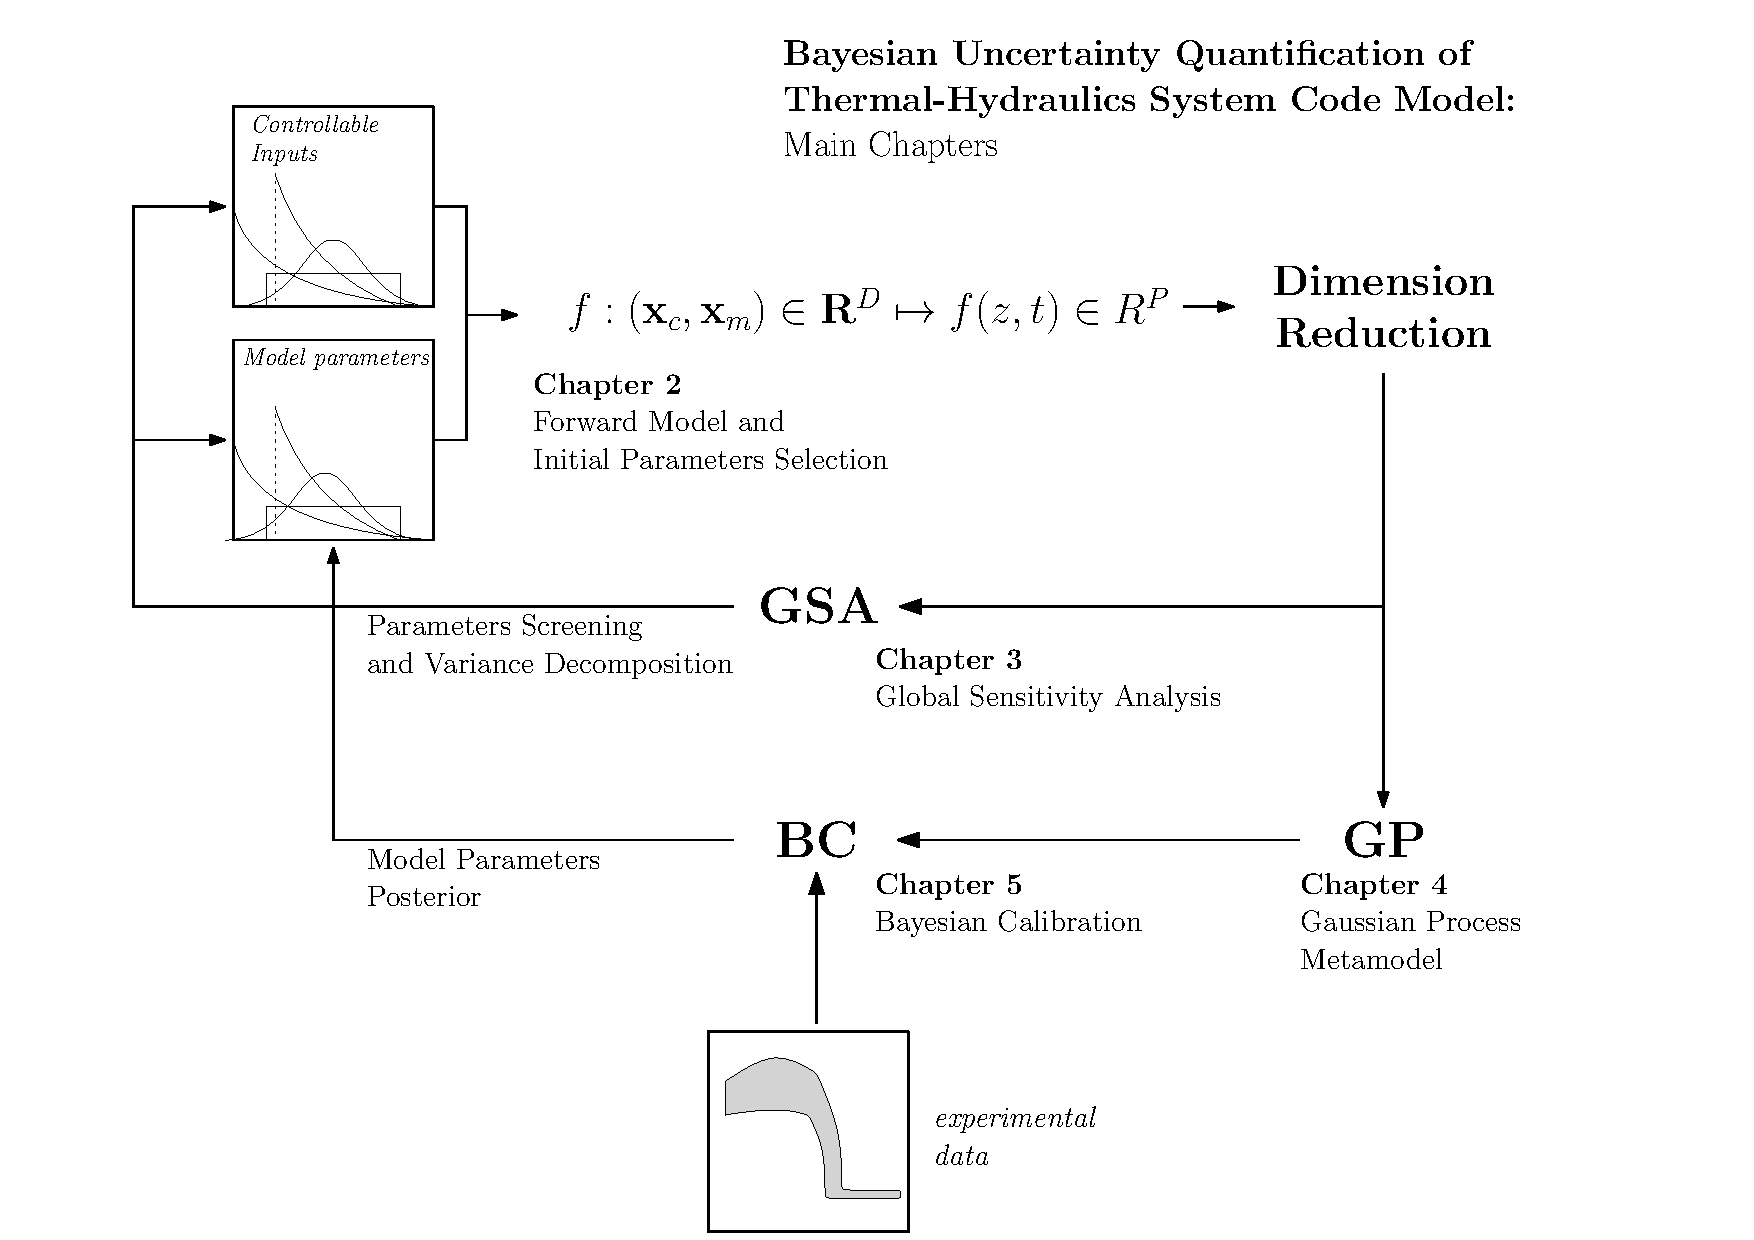
\includegraphics[width=\textwidth]{../figures/chapter1/figures/methodological_roadmap}
	\caption[The structure of thesis.]{The structure of the thesis, its main chapters.}
	\label{fig:ch1_methodological_roadmap}
\end{figure}

\textsc{Chapter~\ref{ch:trace_reflood}} gives an overview of the system thermal-hydraulics code \gls[hyper=false]{trace} with an emphasis on its reflood phenomena modeling and simulation.
The chapter also introduces the reflood experiment at the \gls[hyper=false]{feba} facility which serves as the experimental basis of this work followed by its modeling in \gls[hyper=false]{trace} code.
This model becomes the running example in the three subsequent chapters to which the proposed methods are applied.
The chapter includes the selection of initial parameters relevant for reflood simulation and the propagation of their uncertainties on the code prediction.

\textsc{Chapter~\ref{ch:gsa}} introduces the \gls[hyper=false]{gsa} analysis methods adopted in this thesis with three key underlying ideas.
The first is to reduce the dimensionality of the code output space.
As the output of the simulation is time-dependent, dimension reduction is carried out while trying to preserve the interpretability of the results.
The second idea is to reduce the dimensionality of the input parameters space through parameter screening.
The third and final idea is to investigate, quantitatively, the effect of variation of parameters on the overall time-dependent output variation through variance decomposition.
The presented methods are then applied to the \gls[hyper=false]{trace} model of \gls[hyper=false]{feba} and the results are discussed. 

\textsc{Chapter~\ref{ch:gp_metamodel}} presents the method for model approximation adopted in this thesis.

\textsc{Chapter~\ref{ch:bayesian_calibration}}

\textsc{Chapter~\ref{ch:conclusions}}

%\begin{sidewaysfigure}
%	\centering
%	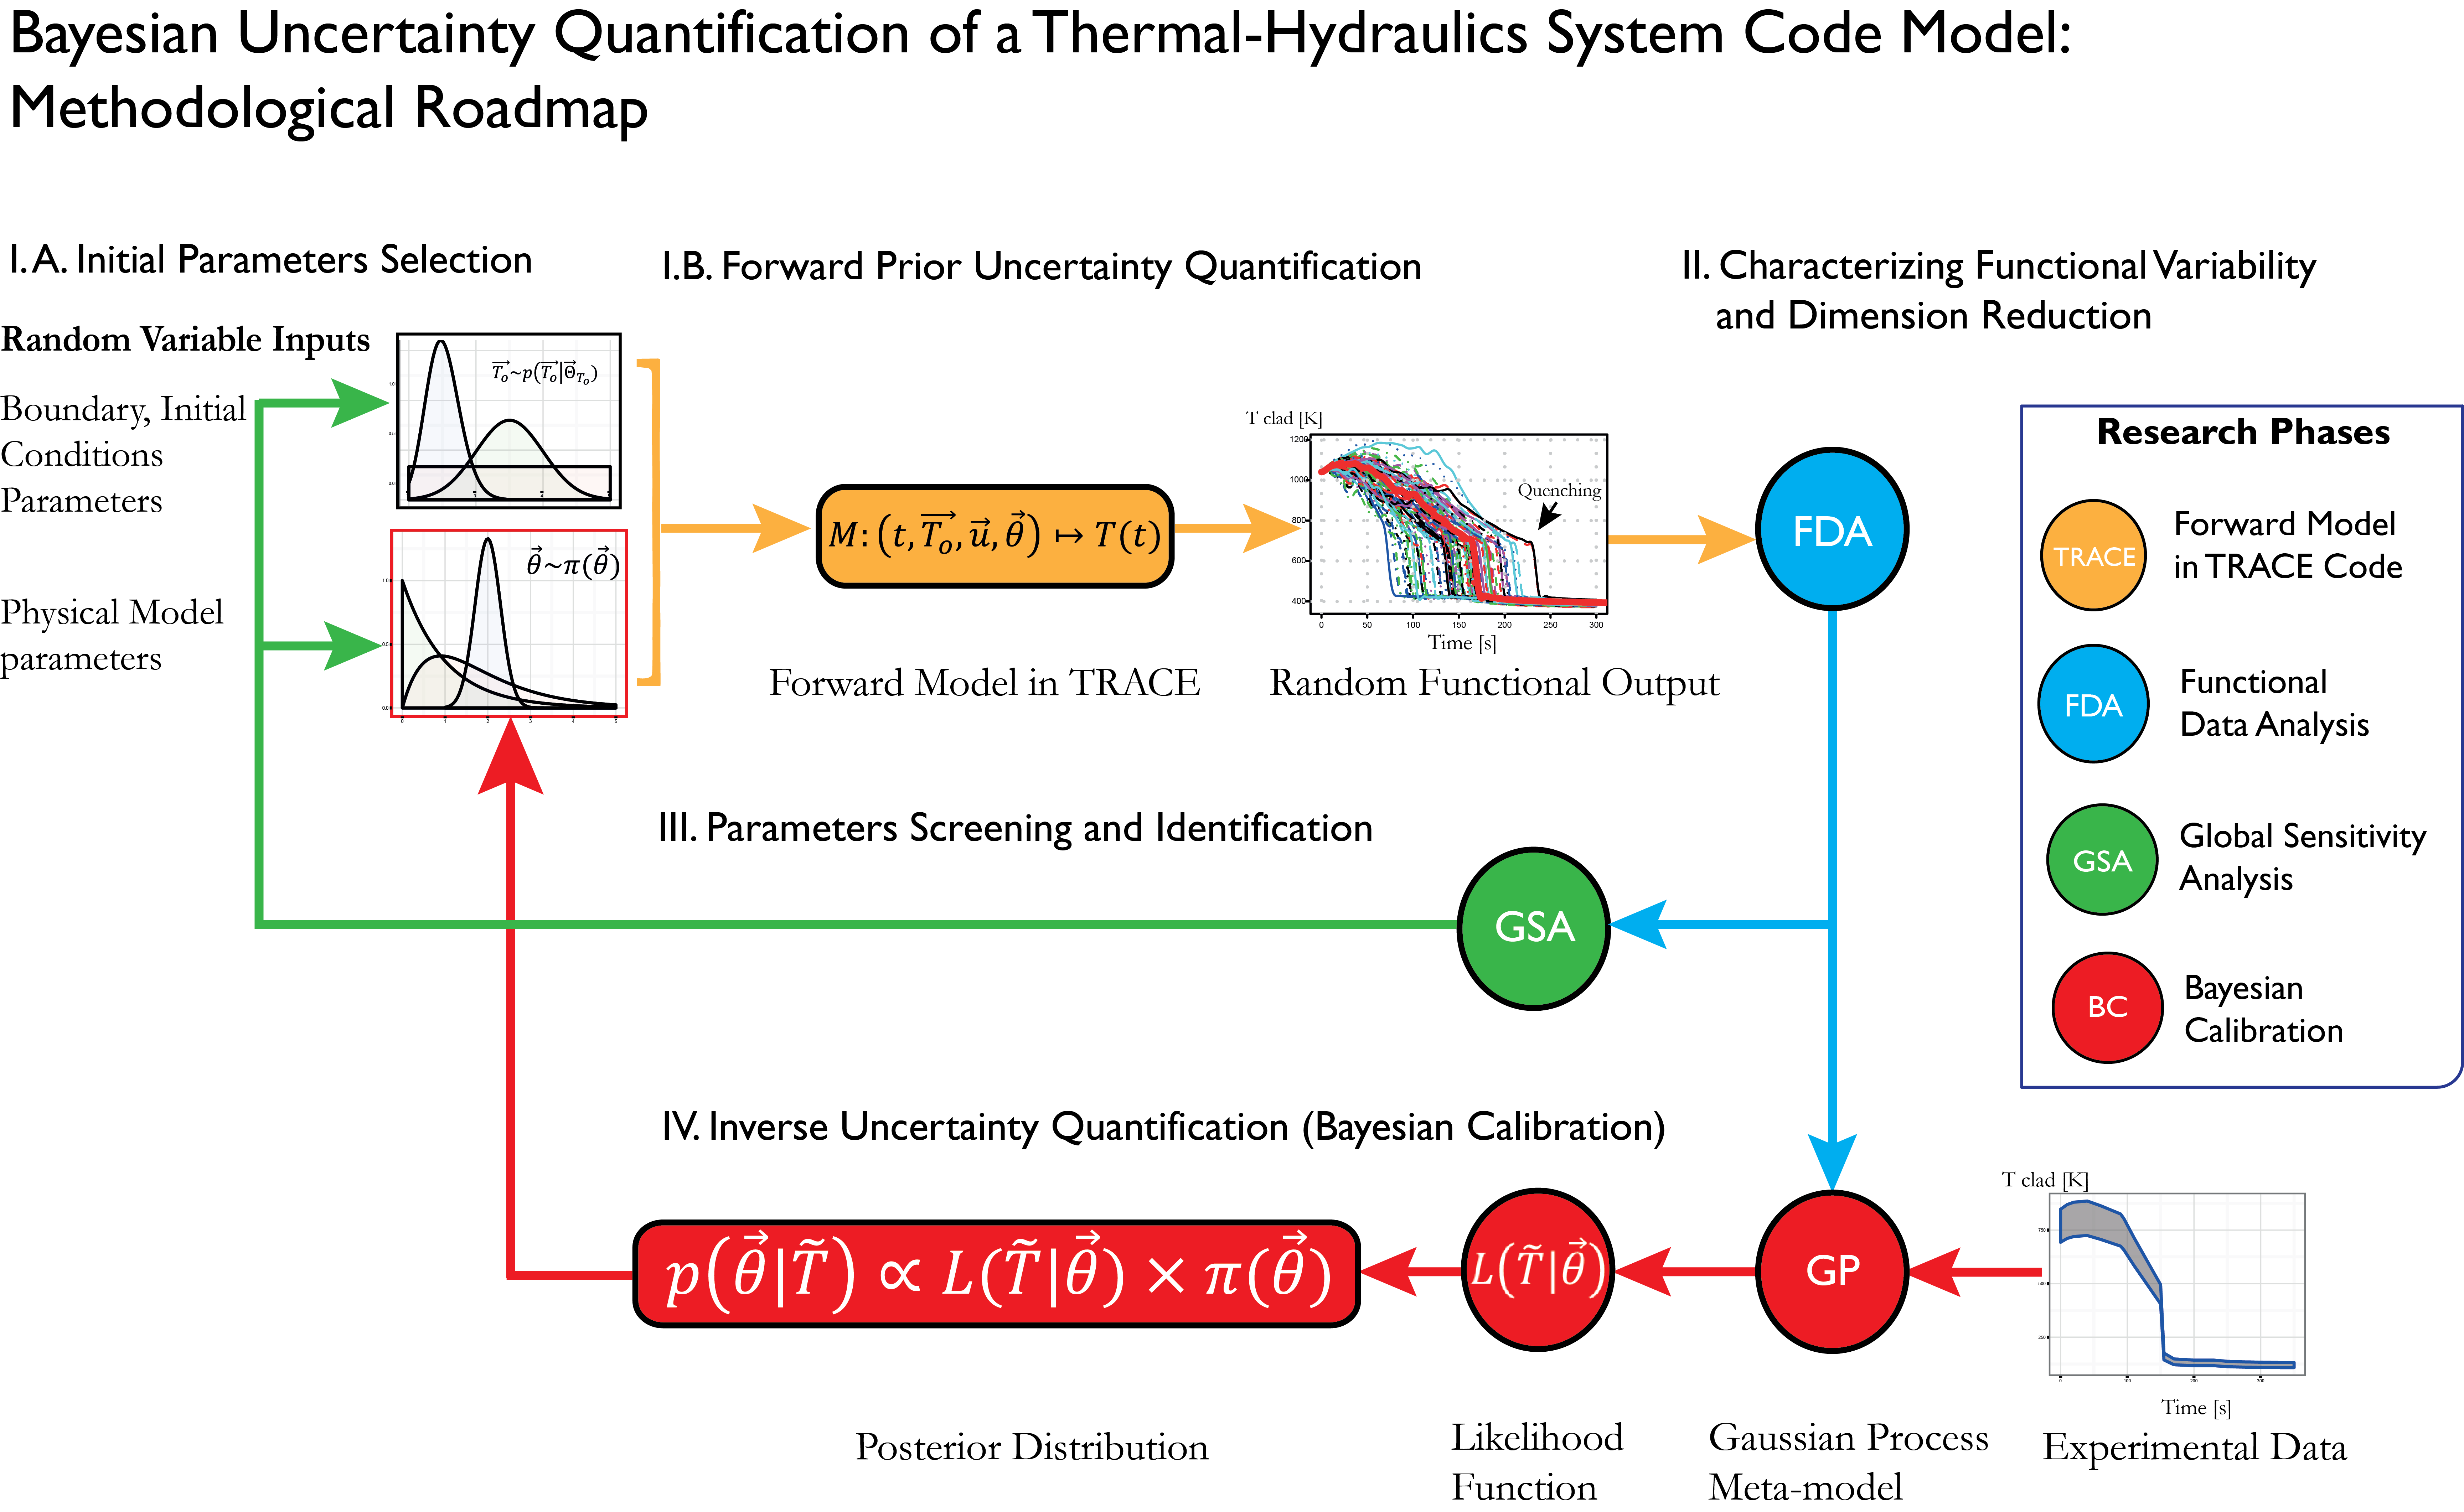
\includegraphics[width=0.85\textwidth]{../figures/methodologicalRoadmap/methodologicalRoadmap.pdf}
%	\caption{Methodological Roadmap of the Thesis}
%	\label{fig:methodological_roadmap}
%\end{sidewaysfigure}